\documentclass[12pt, letterpaper] {article}

\parindent=5mm
\usepackage[spanish]{babel}

\usepackage{amssymb}
\usepackage{amsmath} 
\usepackage{amsfonts}

\usepackage[numbers,sort&compress]{natbib}
\usepackage{graphicx}

\usepackage{url}
\usepackage{hyperref}

\usepackage[top=25mm, bottom=20mm, left=1.5cm, right=1.5cm]{geometry}
\setlength{\parskip}{2mm}
\setlength{\parindent}{1pt}

\usepackage{listings}

\usepackage{float}

\usepackage[utf8]{inputenc}
\usepackage{graphicx} 
\usepackage{subfigure} 

\usepackage{color}
\usepackage{multirow}

\definecolor{dkgreen}{rgb}{0,0.6,0}
\definecolor{gray}{rgb}{0.5,0.5,0.5}
\definecolor{mauve}{rgb}{0.58,0,0.82}

\usepackage{color}
\usepackage{listings}
\lstset{ %
  language=R,                     % the language of the code
  basicstyle=\footnotesize,       % the size of the fonts that are used for the code
  numbers=left,                   % where to put the line-numbers
  numberstyle=\tiny\color{gray},  % the style that is used for the line-numbers
  stepnumber=1,                   % the step between two line-numbers. If it's 1, each line
                                  % will be numbered
  numbersep=5pt,                  % how far the line-numbers are from the code
  backgroundcolor=\color{white},  % choose the background color. You must add \usepackage{color}
  showspaces=false,               % show spaces adding particular underscores
  showstringspaces=false,         % underline spaces within strings
  showtabs=false,                 % show tabs within strings adding particular underscores
  frame=single,                   % adds a frame around the code
  rulecolor=\color{black},        % if not set, the frame-color may be changed on line-breaks within not-black text (e.g. commens (green here))
  tabsize=2,                      % sets default tabsize to 2 spaces
  captionpos=b,                   % sets the caption-position to bottom
  breaklines=true,                % sets automatic line breaking
  breakatwhitespace=false,        % sets if automatic breaks should only happen at whitespace
  title=\lstname,                 % show the filename of files included with \lstinputlisting;
                                  % also try caption instead of title
  keywordstyle=\color{blue},      % keyword style
  commentstyle=\color{dkgreen},   % comment style
  stringstyle=\color{mauve},      % string literal style
  escapeinside={\%*}{*)},         % if you want to add a comment within your code
  morekeywords={*,...}            % if you want to add more keywords to the set
} 
\usepackage{booktabs}
\usepackage[table,xcdraw]{xcolor}
\usepackage{epstopdf}



\author{Ricardo Rosas Macías}

\title{Práctica 7: búsqueda local}

\date{\today}

\begin{document}

\maketitle


\section{Introducción}
La búsqueda local usa el método heur\'istico, que le permite encontrar la mejor soluci\'on de todas las rutas de resultado posibles; a trav\'es de descubrir la posición exacta del agente que le deja obtenerla en un tiempo corto.

 \section{Objetivo}
Se realizó cambios en el c\'odigo proporcionado en la p\'agina web \cite{elisawebBL}\cite{EMP7}, de manera que el agente en el experimento mantiene un movimiento 3D pero con una visualizaci\'on en 2D que permite observar la posici\'on óptima en la secuencia del experimento.
 
 \subsection{Descripción}
 
Lo que se debe hacer es \cite{elisawebBL}:
\begin{quotation}
 ``La finalidad del experimento es maximizar la funci\'on bidimensional del ejemplo $g(x,y)$, con restricciones $-3 \leq x, y \leq 3$, con la misma t\'ecnica del ejemplo unidimensional. La posici\'on actual es un par $x$ y $y$ se ocupan dos movimientos aleatorios, $\vartriangle$$x$ y $\vartriangle$$y$, cuyas combinaciones posibles proveen ocho posiciones vecino, de los cuales aquella que logra el mayor valor para $g$ es seleccionado.\\
El primer reto es cambiar la regla del movimiento de una solución $x$ (un vector de dimensión arbitraria) a la siguiente a la de recocido simulado: para optimizar una función $f(x)$, se genera para la solución actual $x$ un sólo vecino $x'=x+\vartriangle$$x$ (algún desplazamiento local) Se calcula $\delta$$=f(x')-f(x)$ (para minimizar; maximizando la resta se hace al revés). Si $\delta>0$, siempre se acepta al vecino $x'$ como la solución actual ya que representa una mejora. Si $\delta<0$, se acepta a $x'$ con probabilidad $exp(-\frac { \delta  }{ T } )$ y rechaza en otro caso. Aquí $T$ es una temperatura que decrece en aquellos pasos donde se acepta una empeora; la reducción se logra multiplicando el valor actual de $T$ con $\xi<1$, como por ejemplo 0.995. Examina los efectos estadísticos del valor inicial de $T$ y el valor de $\xi$ en la calidad de la solución, es decir, qué tan bajo (para minimizar; alto para maximizar) el mejor valor termina siendo.''
\end{quotation}

\section{Resultados y conclusiones}

En las primeras líneas del c\'odigo se defini\'o los par\'ametros de experimentaci\'on con las cuales se trabajar\'ia con la funci\'on $g$.

\begin{lstlisting}[language=R]
g <- function(x, y) {
  return (((x + 0.5)^4 - 30 * x^2 - 20 * x + (y + 0.5)^4 - 30 * y^2 - 20 * y)/100)
}
low <- -3
high <- -low
step <- 0.25
replicas <- 15
\end{lstlisting}

Posteriormente se gener\'o el c\'odigo que de manera tuviera movimientos de izquierda o derecha, as\'i como con un patr\'on de arriba o abajo, como se muestra en las líneas de c\'odigo. Asimismo, se realizó una combinación de dichos movimientos de modo de recreación de un eje $z$ para el movimiento del agente dentro de la zona creada de $-3 \leq x, y \leq 3$.

\begin{lstlisting}[language=R]
replica <- function(t){
  puntosxy<- c()
  curr <- c( x = runif(1, min = low, max = high), y = runif(1, min = low, max = high))
  best <- curr
  for (tiempo in 1:t) {
    delta <- runif(1, 0, step)
    omega <- runif(1, 0, step)
     left <- curr + c(-delta,0) # Eje izquierdo
    right <- curr + c(delta,0) # Eje Derecho
    up <- curr + c(0,-delta) # Eje arriba
    down <- curr + c(0,delta) # Eje abajo
    puntos <- c(left, right, up, down)

 for(k in 1:8){
      if(puntos[k] < (-3)){
        puntos[k] <- puntos[k]+3 
      }
      if(puntos[k] > 3){
        puntos[k] <- puntos[k]-3
      }
    }
    vecx <- c()
    vecy <- c()
    for(p in 1:8){
      if(p %% 2 == 0){
        vecy <- c(vecy,puntos[p])
      }else{
        vecx <- c(vecx,puntos[p])
      }
    }
    valg <- c()
    for(q in 1:4){
      valg <- c(valg, g(vecx[q], vecy[q]) )
    }
    dm <- which.max(valg)
    curr <- c(vecx[dm], vecy[dm])
    puntosxy <- c(puntosxy, vecx[dm],vecy[dm])
  }
  return(puntosxy)
}

resultado <- c()
for(q in 1:5){
  resultado <- c(resultado, replica(100))
}

vx <- c()
vy <- c()
for(p in 1:1000){
  if(p %% 2 == 0){
    vy <- c(vy,resultado[p])
  }else{
    vx <- c(vx,resultado[p])
  }
}   
\end{lstlisting}

En las l\'ineas finales se puede ver que esta indicado una proximidad m\'axima local para los agentes, lo cual permitir\'a que seleccione el mejor de los vecinos y as\'i este converja en un punto óptimo.

\begin{lstlisting}[language=R]
for (pot in 2:4) {
  tmax <- 10^pot
  resultados <- foreach(i = 1:replicas, .combine="rbind") %dopar% replica(tmax)
  valores <- outer(resultados[,1], resultados[,2], g)
  mejor <- which.max(valores)
  dimnames(valores)<-list(resultados[,1], resultados[,2])
  funcion <- melt(valores)
  names(funcion) <- c("x", "y", "z")
  zona <- levelplot(z ~ x * y, data = funcion)
\end{lstlisting}

Se obtuvieron representaciones gr\'aficas con la ayuda de la paqueter\'ia \textit{lattice} \cite{Lr} de las 15 réplicas simult\'aneas, se seleccionó las mejores representaciones; como se muestra en la figura \ref{GF}, en donde se puede observar que las posiciones iniciales son proporcionadas de manera aleatoria, de modo que con las repéticiones y con un incremento de 10000 en los pasos el resultado se refinó hasta obtener la posici\'on optima del agente, como se puede observar en la figura \ref{Rep5}.

\begin{figure}[H]
\centering
\subfigure[Repetici\'on 1]{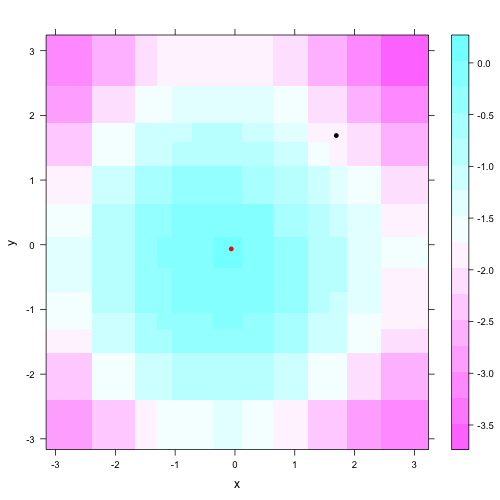
\includegraphics[width=65mm]{./10000pasosen1rep}}\vspace{1mm}
\subfigure[Repetici\'on 2]{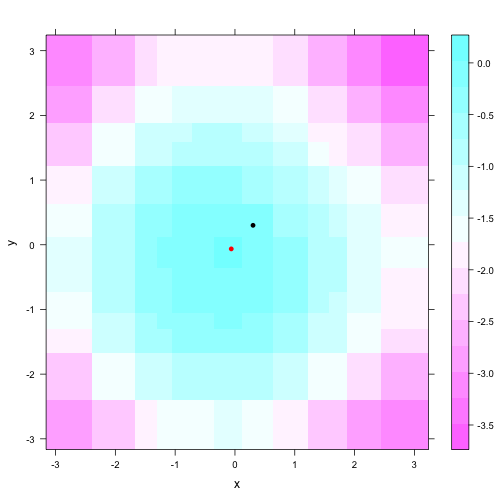
\includegraphics[width=65mm]{./10000pasosen2rep}}
\subfigure[Repetici\'on 3]{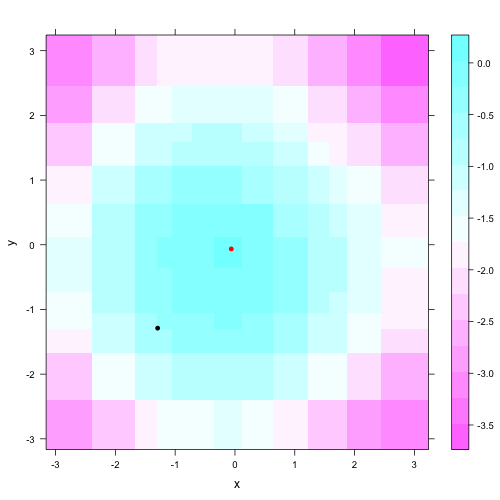
\includegraphics[width=65mm]{./10000pasosen3rep}}
\subfigure[Repetici\'on 5]{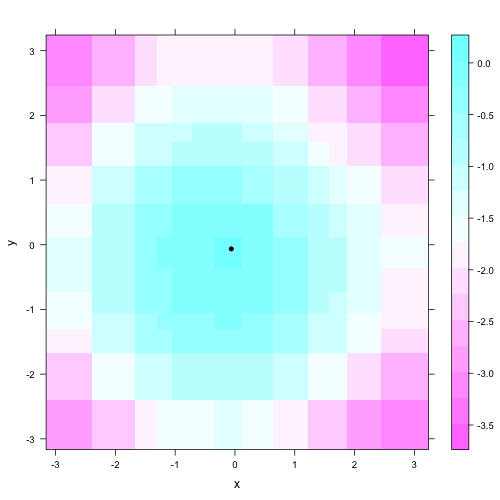
\includegraphics[width=65mm]{./10000pasosen5rep}\label{Rep5}}
\caption{Proyecci\'on plana del experimento a 10000 pasos}\label{GF}
\end{figure}

\subsection{Reto1}
Para realizar el reto 1, se tomo como ejemplo lo anteriormente reportado \cite{P7RCP}, como se muestra en las líneas siguientes. 

\begin{lstlisting}[language=R]
g <- function(x, y) {
  a<- (((x + 0.5)^4 - 30 * x^2 - 20 * x + (y + 0.5)^4 - 30 * y^2 - 20 * y)/100)
  return(a)
}
valeng <- c()
temperaturas <- c(5,10,15,20,40)
for(tem in temperaturas){
  low <- -3
  high <- -low
  step <- 0.25
  replicas <- 15
  t <- tem
  ep <- 0.80
  replica <- function(t){
    curr <- c(runif(1, low, high), runif(1, low, high))
    best <- curr
    for (tiempo in 1:t) {
      delta <- runif(1, 0, step)
      x1 <- curr + c(-delta,0)
      x2 <- curr + c(delta,0)
      y1 <- curr + c(0,-delta)
      y2 <- curr + c(0,delta)
      puntos <- c(x1,x2,y1,y2)
      for(k in 1:8){
        if(puntos[k] < (-5)){
          puntos[k] <- puntos[k]+10
        }
        if(puntos[k] > 5){
          puntos[k] <- puntos[k]-10
        }
      }
      vecx <- c()
      vecy <- c()
      for(p in 1:8){
        if(p %% 2 == 0){
          vecy <- c(vecy,puntos[p])
        }else{
          vecx <- c(vecx,puntos[p])
        }
      }
      u <- sample(1:4,1)
      x.p <- c(vecx[u],vecy[u])
      delt <- g(x.p[1],x.p[2]) - g(curr[1],curr[2])
      if(delt > 0){
        curr <- x.p
      }else{
        if(runif(1)< exp((delt) / (t * ep))){
          curr <- x.p
          if(t == 1){
            t <-t
          }else{
            t <- t-1
          }
        }
      }
      if(g(curr[1],curr[2]) > g(best[1],best[2])){
        best <- curr
      }
    }
    return(best)
  }
  tmax <- 100
  resultados <- c()
  for(indi in 1:100){
    resultados <- c(resultados, replica(tmax))
  }
  vecx <- c()
  vecy <- c()
  aux <- 200
  for(p in 1:aux){
    if(p %% 2 == 0){
      vecy <- c(vecy,resultados[p])
    }else{
      vecx <- c(vecx,resultados[p])
    }
  }
  valores <- c()
  for(q in 1:100){
    valores <- c(valores, g(vecx[q], vecy[q]))
  }
  valeng <- c(valeng, valores) 
}
\end{lstlisting}

En la figura \ref{FRSS} se puede observar el valor del recocido a diferentes temperaturas a un valor de $\xi$ de 0.1, en donde se puede determinar que la temperatura no altera el resultado final, debido a que hay una diferencia despreciable como se muestra en las cajas bigote. 

\begin{figure}[H]
\centering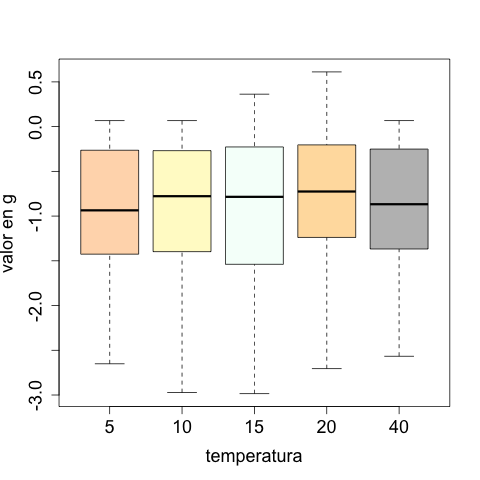
\includegraphics[width=98mm]{Dimarb.png}
\caption{Resultados de recocido simulado}
\label{FRSS}
\end{figure}

\bibliographystyle{plainnat}

\bibliography{BHWP7}

\end{document} 